\section{Alert Production}
\label{sec:ap}



Alert Production is run each night to product catalogs and images for sources that have varied or moved relative to a previous observation.  The data products produced by Alert production are given in  table~\ref{table:ap_data_products}.

\begin{table}
\small
\begin{tabularx}{\textwidth}{ | l | l | X | }
  \hline
  {\bf Name} & {\bf Availability} & {\bf Description} \\
  \hline
  DIASource & Stored &
  Measurements from difference imagine analysis of individual exposures. \\
  \hline
  DIAObject& Stored &
  Aggregate quantities computing by associating spatially colocated DIASources. \\
  \hline
  DIAForcedSource & Stored &
  Flux measurements on each difference image at the position of every DIAObject. \\
  \hline
  SSObject & Stored &
  Solar system objects derived by associating DIASources and inferring their orbits. \\
  \hline
  CalExp & Stored &
  Calibrated exposure images for each CCD/visit (sum of two snaps). \\
  \hline
  DiffExp & Stored &
  Difference between CalExp and PSF-matched template coadd. \\
  \hline
\end{tabularx}
\caption{Table of derived and persisted data products produced during a Alert Production.  A description of these data products can be found in the Data Products Definition Document (LSE-163).
\label{table:ap_data_products}}
\end{table}


Alert Production is designed as five separate components: single frame
processing, alert detection, alert generation, precovery photometry,
and a moving objects pipeline. The first four of these components run
as a linear pass through of the data. The moving objects pipeline is
run independently of the rest of the alert production. The flow of
information through this system is shown in figure~\ref{fig:nightly}.

\begin{figure}[th]
\begin{center}
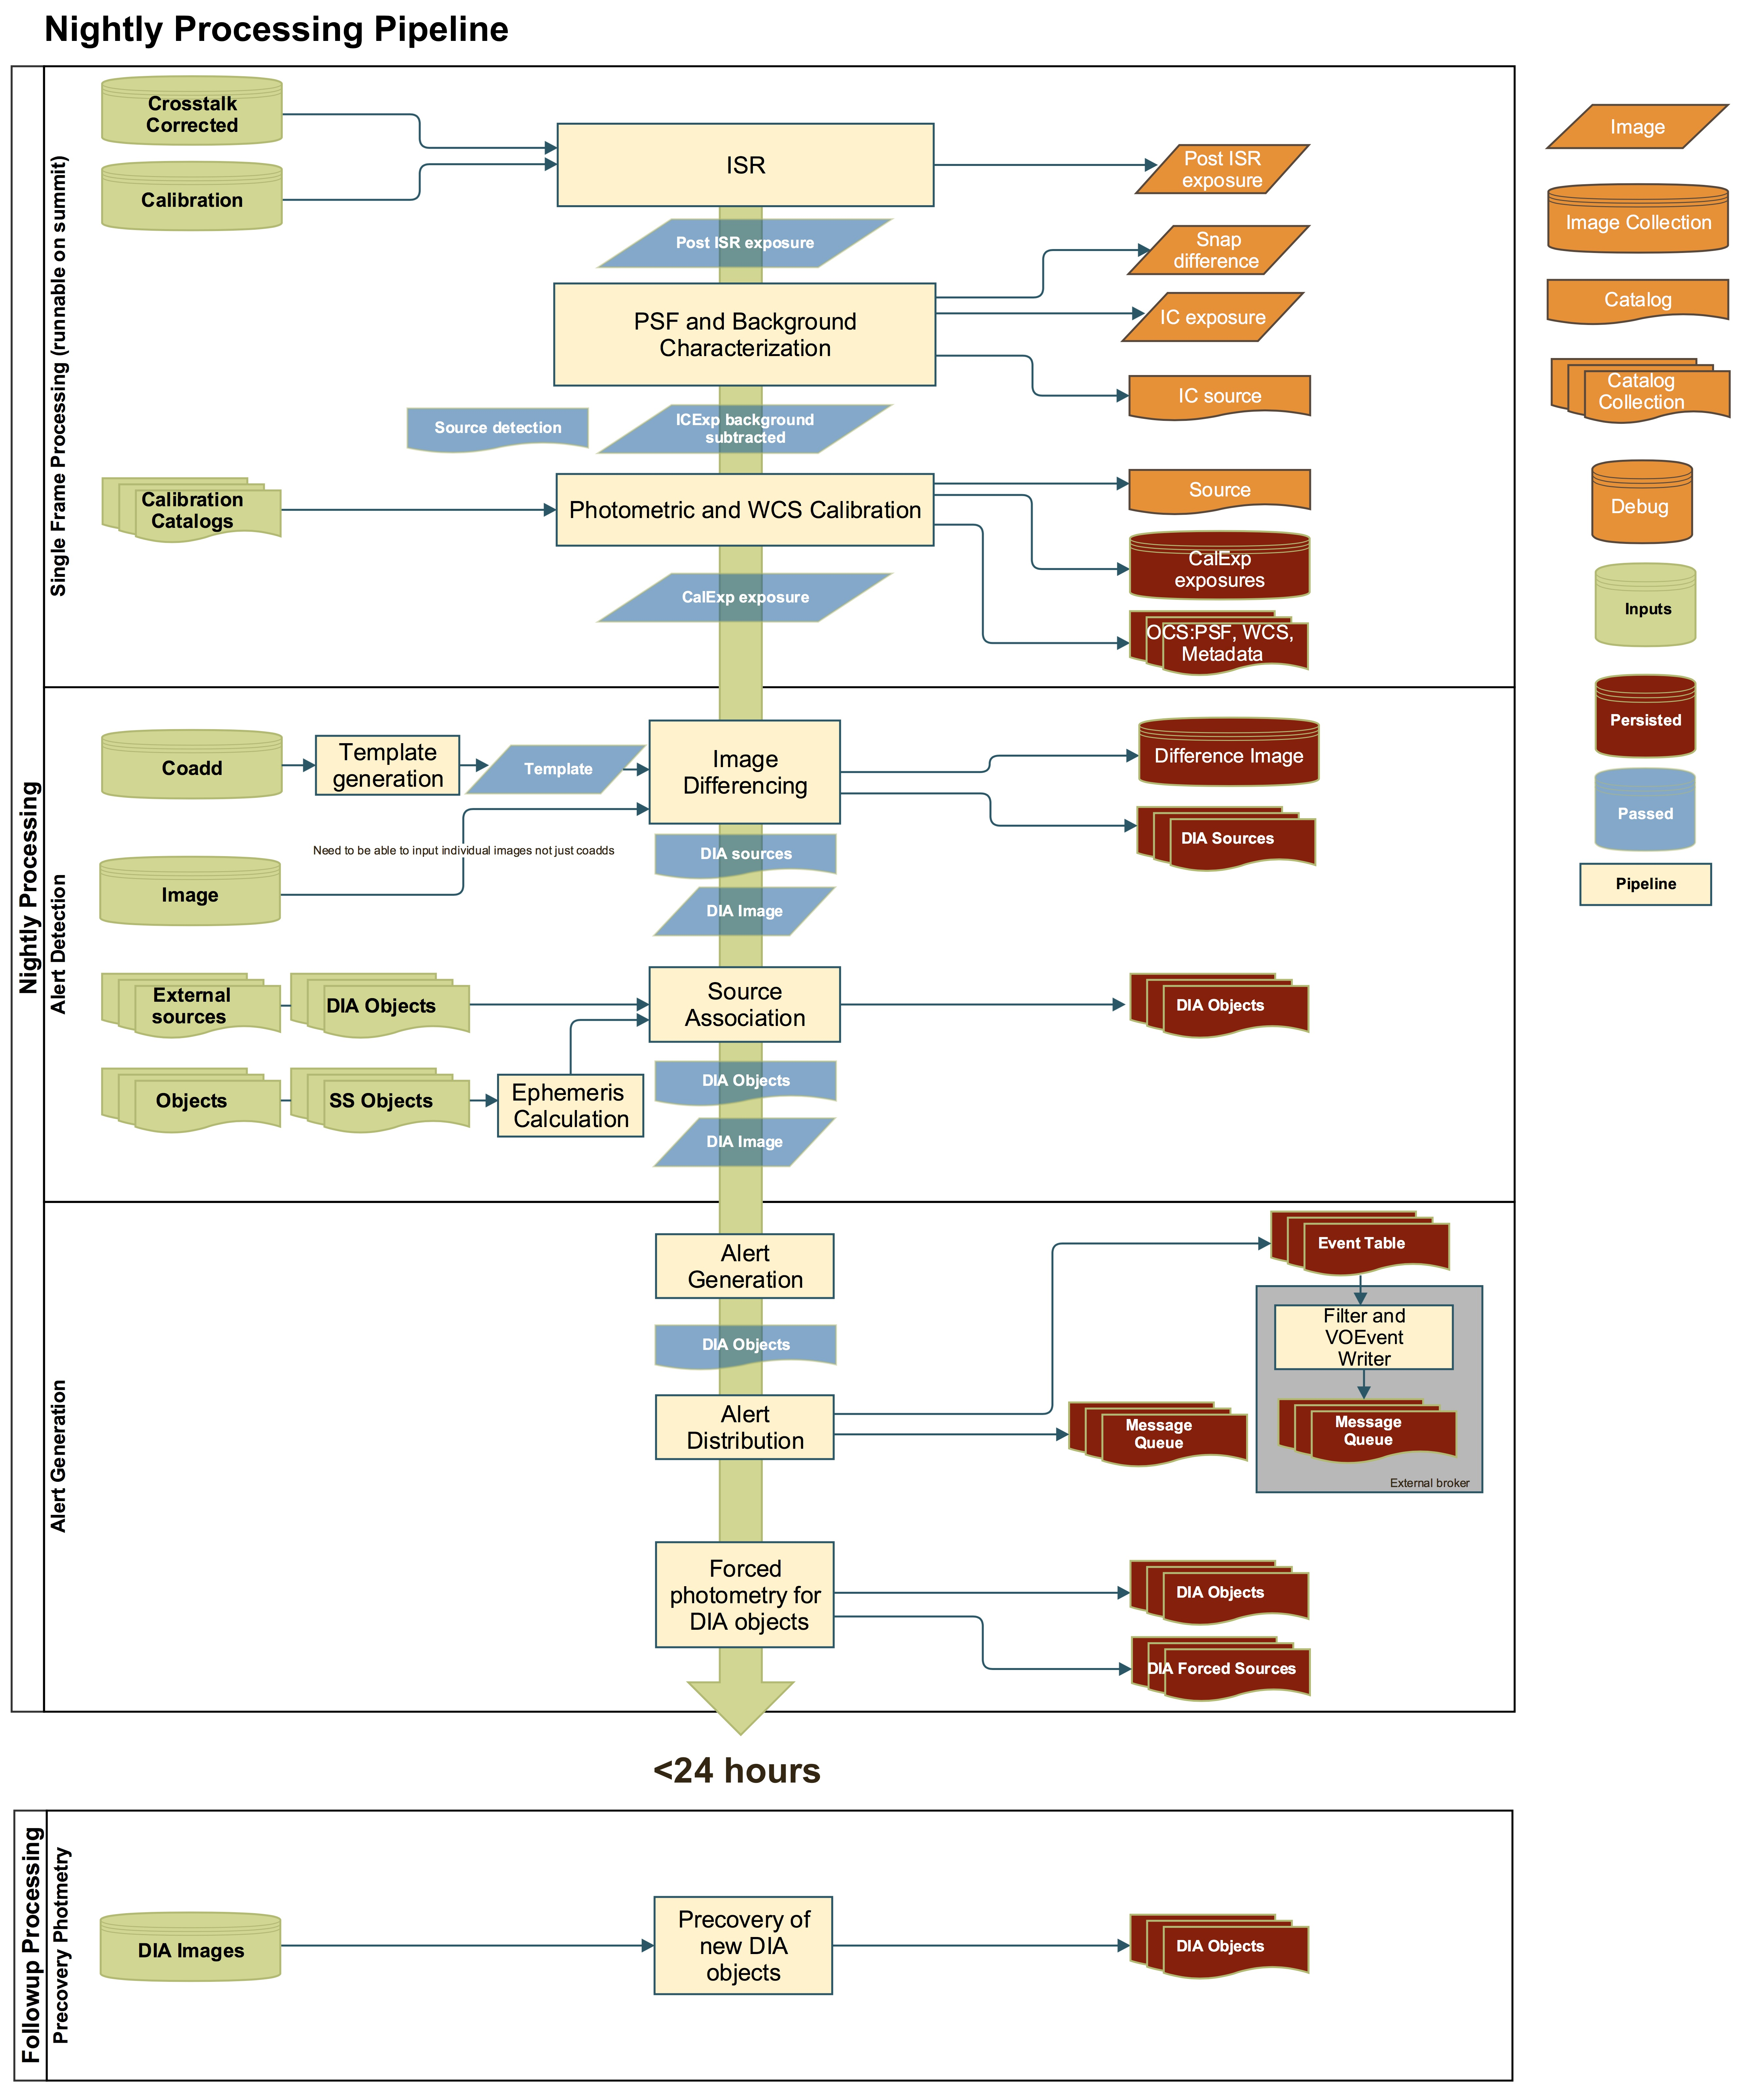
\includegraphics[width=0.9\textwidth]{figures/Level_1_Processing_Flowchart.jpg}
\caption{\label{fig:nightly} The alert production flow of data through
  the processing pipelines (single frame processing, alert detection,
  alert generation, precovery photometry) }
\end{center}
\end{figure}

\subsection{Single Frame Processing Pipeline (\wbsSFM)}
\label{sec:apSingleFrameProcessing}

Single Frame Processing (SFM) Pipeline is responsible for reducing raw or camera corrected image data to \emph{calibrated exposures}, the detection and measurement of \Sources (using the components functionally a part of the Object Characterization Pipeline), the characterization of the point-spread-function (PSF), and the generation of an astrometric solution for an image.

\subsubsection{Baseline Design}

Single Frame Processing pipeline will be implemented as a flexible   framework where new processing steps can be added without modifying the stack code. It should be possible for this pipeline or a subset of this pipeline  to be run at the telescope facility during commissioning and operations.  

\paragraph{Input Data: Raw}

Amplifier images that the camera has corrected for crosstalk, overscan, linearity.  All images from a visit should be available to the task (including snaps). An approximate WCS is assumed to be available as metadata

\paragraph{Input Data Product: Reference}

A full-sky reference catalog of stars derived either from an external survey (e.g.\ Gaia) or from the Data Release Processing.

Flatfield calibration images for all passbands and all CCDs appropriate for the time at which the observations were undertaken

List of the positions and extents of sensor defects for all CCDs within the focal plane

Metadata for all CCDs including electronic parameters (saturation limits, readnoise, electronic footprint)

\paragraph{Output Data Product: CalExp}

A calibrated exposure (CalExp).  CalExp is an \hyperref[sec:spImagesExposure]{Exposure} object. The CalExp will contain a PSF, WCS, PhotoCalib and Background. The pixel data will include the image, mask, and variance. 

\paragraph{Output Data Product: Source}

A catalog of Sources with measured features (as described in \ref{sec:ac}). 


\paragraph{Output Data Product: Metadata}
A parameterization of the PSF for the visit, the WCS for the visit,
and associated metadata (e.g.\ photometric depth) must be made
available to the telescope Observatory Control System (OCS). It is
expected that these data will be persisted within a database that will
be queried by the OCS.


SFM pipeline functions include:
\begin{itemize}
\item Assembly of per-amplifier images to an image of the entire CCD;
\item Instrumental Signature Removal;
\item Cosmic ray rejection and snap combining;
\item Per-CCD determination of zeropoint and aperture corrections;
\item Per-CCD PSF determination;
\item Per-CCD WCS determination and astrometric registration of images;
\item Per-CCD sky background determination;
\item Source detection and measurement on single frame images
\item Generation of metadata required by the OCS
\end{itemize}

Calibrated exposure produced by the SFM pipeline must possess all information necessary for measurement of source properties by single-epoch Object Characterization algorithms.

\paragraph{Actions in case of failure:}

In the case camera data are not available due to a network outage that is longer than the data buffer at the summit the single frame processing will work on raw images (i.e.\ without the camera pixel corrections) and be run in a batch mode. 



\paragraph{Instrumental Signature Removal:}~
\label{sec:apISR}
Instrumental Signature Removal characterizes, corrects, interpolates
and flags the camera (or raw) images to generate a flat-fielded and corrected
exposure.

\paragraph{Pipeline Tasks}
\begin{itemize}
\item Mask CCD defects based on the and saturation
\item Assembly
\item Full frame corrections: Dark, Flats (includes fringing)
\item Pixel level corrections: Brighter fatter, static pixel size effects
\item Interpolation of defects and saturation
\item \hyperref[sec:artifact]{CR rejection}
\item Generate snap difference
\item Snap combination
\end{itemize}


\paragraph{PSF and background determination:}~
\label{sec:apPSFBackground}

Given exposures that have been processed through the Instrument Signature Removal, sources must be detected that will be used to determine the WCS and photometric calibration of the images. Detection and measurement of the properties of these calibration Sources requires knowlege of the PSF and background for the image which in turn requires knowledge of the sources on the image. An iterative procedure is, therefore, adopted to generate the Source catalog. 

\paragraph{Pipeline Tasks}
The procedure for PSF and background estimation and the associated
algorithmic components. Convergence criteria for the procedure is not
defined but the default procedure assumes three iterations.
\begin{itemize}
\item \hyperref[sec:acBackgroundEstimation]{Background estimation}
\item \hyperref[sec:acSourceDetection]{Source detection} to the 5$\sigma$ limit of
%\item Single CCD \hyperref[sec:acDeblending]{Deblend sources}
\item Selection of PSF candidate stars based on a signal-to-noise threshold 
  (default 50 $\sigma$) and isolated sources 
\item Single CCD \hyperref[sec:acSingleCCDPSF]{PSF determination} given the selected bright sources
%\item Single CCD \hyperref[sec:acModelSpatialPSF]{PSF spatial model}
\end{itemize}


\paragraph{Source measurement:}~
\label{sec:apSourcemeasurement}

For the Source catalog generated in \label{sec:apPSFBackground} measure the source properties using a subset of features measured in \label{sec:drpMeasureSources}. Source measurement if for all sources within the Source catalog and not just the bright subset used to calibrate the PSF. 

\paragraph{Pipeline Tasks}
We anticipate using the following plugin algorithms for \label{sec:drpMeasureSources}
\begin{itemize}
\item \hyperref[sec:acCentroidAlgorithms]{Centroids}
\item \hyperref[sec:acPixelFlags]{Pixel Flag Aggregation}
\item \hyperref[sec:acAperturePhotometry]{Aperture Photometry} (but only for one or two radii) 
\item \hyperref[sec:acPSFPhotometry]{PSF Photometry} 
\item \hyperref[sec:acStaticPointSourceModels]{Static Point Source Models}
\item  \hyperref[sec:apertureCorrection]{Aperture correction} for  detected sources
\end{itemize}

\paragraph{Photometric and Astrometric calibration:}~
Photometric and astrometric calibration entails a ``semi-blind'' cross match of a reference catalog (derived either from the DRP Objects or from an external catalog), the generation of a WCS (on the scale of a CCD or visit), and the generation of a photometric zeropoint (on the scale of a CCD).

\paragraph{Pipeline Tasks}
Photometric and astrometric calibration performed at the scale of a
single sensor (extended to the scale of a visit depending on required fidelity)
\begin{itemize}
\item CCD level \hyperref[sec:acSingleCCDReferenceMatching]{source
    association} between the DRP reference catalog and Sources from the \ref{sec:apSourcemeasurement}
\item Generation of a \hyperref[sec:acSingleCCDPhotometricFit]{photometric solution} at the level of a single CCD
\item Decomposition of the astrometric components (e.g.\ optical distortions, sensor tree-rings) for a single CCD and generation of an \hyperref[sec:acSingleCCDAstrometricFit]{astrometric fit} at the level of a single CCD
\item Persistence of the astrometric, PSF, and photometric solutions so that the OCS can incorporate it into their telemetry
\end{itemize}

Given the number of stars available on a CCD or the complexity of the astrometric solutions for the LSST it may be necessary that the astrometric and photometric solutions must be performed at the level of a visit and not a CCD.  For these cases the operations will be \hyperref[sec:acSingleVisitReferenceMatching]{single visit matching},   \hyperref[sec:acSingleCCDPhotometricFit]{single visit photometric solutions}, \hyperref[sec:acSingleVisitAstrometricFit]{single visit astrometric fits}.

Astrometric and photometric performance within crowded fields will require that the order of the WCS should depend on the number of calibration Sources that are available.

\clearpage

\subsection{Alert Detection (\wbsDiffim)}
\label{sec:apAlertDetection}

\noindent 
{\bf Input Data:}\\
\begin{itemize}
\item Butler access to Coadd images from DRP that overlap spatially
  with CalExp images 
\item Access to DIAObjects that overlap spatially with CalExp images 
\item Access to Objects that overlap spatially  with CalExp images 
\item Access to SSObjects whose ephemerides overlap spatially  with CalExp images 
\item Internal reference catalog for CalExp from DRP 
\item PSF \hyperref[sec:apSingleFrameProcessing]{measured} from the
  science image.
\item Data structures for the real-bogus classifier
\end{itemize}


{\bf Output Data}\\
\begin{itemize}
\item DIAimage persisted
\item DIASources persisted
\item DIAObjects persisted
\item DIA forced photometry persisted
\end{itemize}

{\bf Actions in case of failure:}\\
{\bf Alternative procedures:}\\
\begin{itemize}
\item Butler access to CalExp images from DRP that overlap spatially
  with current CalExp image  for template generation
\end{itemize}
\subsubsection{Key Requirements}

The alert detection pipeline shall difference a visit image against a deeper template, and detect and characterize sources in the difference image in the time required to achieve the 60 second design goal for Level 1 alert processing (current timing allocation: 24 seconds). The algorithms employed by the pipeline shall result in purity and completeness of the sample as required by the \DMSR\@. Image differencing shall perform as well in crowded as in uncrowded fields.

\subsubsection{Baseline Design}
\label{sec:diffimDesign}

\paragraph{Template Generation}~

By either querying for Coadd Images that spatially overlap with a
given CalExp or for a DCR differential chromatic refraction corrected
template (see \hyperref[sec:acRetrieveTemplate]{Retrieve Diffim
  Template}) template image.

\noindent
{\bf Subtasks:}
\begin{itemize}
\item Query for Coadd images that are within a given time interval
  (default 2 years) of the current sensor image, and are within
  allowable airmass limits (default XXX). seexs
  \hyperref[sec:acRetrieveTemplate]{template retrieval}
\item An alternate approach will be to return an interpolated,
  DCR-corrected template based on a model of the effect of DCR (see
  \hyperref[sec:acDCRTemplates]{ DCR template generation}). The
  direction of the DCR correction will be aligned with the 
  ``parallactic angle''.
  \end{itemize}

\paragraph{Image differencing}~

Model the matching kernel and its spatial variation using a regression
approach and a \hyperref[sec:acImageSubtraction]{set of basis functions}

\noindent
{\bf Subtasks:}
\begin{itemize}
\item Match \hyperref[sec:apSourcemeasurement]{DRP} sources and
  sources from \hyperref[sec:apSingleFrameProcessing]{SFP}
\item Determine a relative astrometric solution
\item Warp the template and measurements to the science image frame
\item Determine the appropriate PSF matching sources
\item Decorrelate the science image with an estimate of the science PSF (pre-convolution) 
\item Compute the PSF matching kernel and spatial model using
  \hyperref[sec:acDiffImDecorrelation]{ZOGY} approach
\item Difference the science and template images
\item Apply a correction for correlated noise
\item Difference image \hyperref[sec:acSourceDetection]{source
    detection} to generate DIASources
\item Difference image  \hyperref[sec:acMeasurement]{source
    measurement}: \hyperref[sec:acDipoleModels]{dipole fit}, \hyperref[sec:acTrailedPointSourceModels]{trailed source} measurement
\item Measure flux on snap difference for all DIASources
\end{itemize}

\paragraph{Real-Bogus classification}~

Initial classification step to identify false positives in the image
difference sources. Training of the classifier will be undertaken
outside of the nightly processing and will utilize a training sample
of real variable sources and artifacts based on labelled data. Labels
will be derived from simulated data and visually classified sources.

\noindent
{\bf Subtasks:}
\begin{itemize}
\item The data structures for the real-bogus machine learning
  algorithm(s) will be loaded
\item A random forest or other probabilistic classification algorithm will be
  applied to the DIASources
\item Update the DIASources with the probabilistic classification 
\item Prune the DIASource list based on classifier results
\end{itemize}

\paragraph{Source Association}~

{\bf Input Data:}\\
\begin{itemize}
\item Access to DIAObjects and that overlap spatially with CalExp images
\item Access to Objects that overlap spatially  with CalExp images
\item Access to SSObjects whose \hyperref[sec:acEphemerisCalculation]{ephemerides} overlap spatially with CalExp images
\item Internal reference catalog for CalExp from DRP
\item PSF \hyperref[sec:apSingleFrameProcessing]{measured} from the
  science image
\item Data structures for the real-bogus classifier
\end{itemize}


{\bf Output Data}\\
\begin{itemize}
\item DIAimage persisted
\item DIASources persisted
\item DIAObjects persisted
\item DIA forced photometry persisted
\end{itemize}
\noindent
{\bf Subtasks:}
\begin{itemize}
\item Given the time of an observation and the motion of the sources,
  propagate positions of all sources (SSObjects and DIASources).
\item Using the WCS determine the sensor coordinates for all
  DIAObjects in the catalog
\item Match all DIASources to all DIAObject catalog positions using a probabilistic \hyperref[sec:acDIAObjectGeneration]{matching algorithm}
\item Update associated DIAObjects with aggregate quantities
  e.g. position and flux (in a 30 day rolling wind)
\item Perform forced photometry of all DIAObjects that intersect with
  the frame.
\end{itemize}


\subsubsection{Prototype Implementation}

The prototype code is available at \url{https://github.com/lsst/ip_diffim}. The current prototype, while functional, will require a partial redesign to be transfered to construction to address performance and extensibility concerns.

\clearpage

\subsection{Alert Generation Pipeline (\wbsAP)}

\subsubsection{Key Requirements}

Alert Generation Pipeline shall take the newly discovered \DIASources and all associated metadata as described
in the \DPDD, and deliver alert packets in \VOEvent format to a variety of endpoints via standard IVOA protocols (eg., VOEvent Transport Protocol; VTP\@).

To directly serve the end-users, the Alert Generation Pipeline shall provide a basic, limited capacity, alert filtering service. This service will run at the LSST U.S. Archive Center (at NCSA). It will let astronomers create simple filters that limit what alerts, and what fields from those alerts, are ultimately forwarded to them. These \emph{user defined filters} will be possible to specify using an SQL-like declarative language, or short snippets of (likely Python) code.

Since there is a need to keep both the alert database and the brokers consistent, there is a big win if both the database and the brokers read from the same fault tolerant intermediate persistence format.  A redundant, cluster based, strongly ordered, message system like Kafka (http://kafka.apache.org) is a very attractive option as the intermediate persistence.  It is very similar in concept to persisting to some well known file format with the addition of reduntant storage, configurable expiration time of messages, and strict ordering so database catch-up is trivial.  It is also scalable.

\subsubsection{Baseline Design}

{\bf Input Data:}\\
\begin{itemize}
\item Access to DIAObjects that overlap spatially with CalExp images
\item Access to Template image that overlap spatially with CalExp images
\end{itemize}


{\bf Output Data}\\
\begin{itemize}
\item DIA event table persisted
\item VOEvents
\end{itemize}

\paragraph{Alert generation}~

\noindent
{\bf Subtasks:}
\begin{itemize}
\item Generate postage stamps for all DIASources: direct image and difference image
\item Push alert records to alert persistence
\item Alert database ingestion client reads all new alerts and persists them permanently in the alert database
\end{itemize}

\paragraph{Alert Distribution: To community brokers}
\noindent
{\bf Subtasks:}
\begin{itemize}
\item For each visit read all new alert records from the alert persistence
\item Package each message as a properly formatted VOEvent
\item Bundle VOEvents using a pre-negotiated format
\item Transmit bundled VOEvents to community broker endpoints
\end{itemize}

\paragraph{Alert Distribution: Minimal brokers}
\noindent
Each minimal broker will have some subset of users.  The following is for a single broker.
{\bf Subtasks:}
\begin{itemize}
\item Read new alert records from the alert persistence in order
\item Filter event records for relevance (WHERE)
\item Filter event columns for content (SELECT)
\item Package event as a valid VOEvent
\item Publish the VOEvent to the appropriate endpoint (potentially another messaging queue so clients can access asynchronosly)
\end{itemize}

\paragraph{Forced Photometry on all DIAObjects}~

\noindent
{\bf Subtasks:}
\begin{itemize}
\item Compute forced photometry on all DIAObjects in the field.  This
  does not end up in the alerts.
\item Update the DIA Object forced photometry tables
\end{itemize}

\subsubsection{Prototype Implementation}

\clearpage

\subsection{Precovery Photometry Pipeline}

\noindent
{\bf Input Data:}\\
\begin{itemize}
\item Butler access to DIA images within finite time interval (default 
  30 days) 
\item Butler access to DIAobjects detected from the previous night 
  with no associations 
\end{itemize}
{\bf Output Data}\\
\begin{itemize}
\item Updated and persisted forced photometry tables for all newly
  detected DIAobjects
\end{itemize}

\subsubsection{Key Requirements}

Within 24 hrs.

\paragraph{Precovery of new DIAObjects}~

\noindent
{\bf Subtasks:}
\begin{itemize}
\item Force photometer in difference images for all new DIAObjects for the past 30 days.
\end{itemize}
\clearpage

\subsection{Moving Object Pipeline (\wbsMOPS)}

\subsubsection{Key Requirements}

The Moving Object Pipeline is responsible for generating and managing the Solar System\footnote{Also sometimes referred to as `Moving Object'} data products. These are Solar System objects with associated Keplerian orbits, errors, and detected \DIASources. Quantitatively, it shall be capable of detecting 95\% of all Solar System objects that meet the findability criteria as defined in the \OSS\@. 

\subsubsection{Baseline Design}
{\bf Input Data}\\
\begin{itemize}
\item 'Orphan' DIASources from the last night of observing.  This means DIASources that are not associated with a DIAObject.  DIASources associated with an SSObject in the night are still passed through the MOPS machinery
\item DIAObject database
\item SSObject database
\item Exposure metadata database
\end{itemize}
{\bf Output Data}\\
\begin{itemize}
\item Updated SSObject databaase
\item Updated DIASource database
\end{itemize}
{\bf Anscillary Products}\\
\begin{itemize}
\item Tracklet database
\item Track database
\item Intermediate orbit prediction database
\end{itemize}
{\bf Actions in case of failure}\\
{\bf Alternative procedures}\\

{\bf Subtasks:}
\begin{itemize}
\item Feed all input orphan DIASources to \hyperref[sec:acMakeTracklets][makeTracklets].
\item Run \hyperref[sec:acAttributionAndPrecovery]{attribution and precovery} on with just the tracklets and DIASources from the previous night.  This culls any tracklets or DIASources that obviously belong to an existing SSObject from the rest of the processing.
\item Compute new \hyperref[sec:acOrbitFitting]{orbits} and \hyperref[sec:acOrbitMerging]{merge orbits}.
\item Run \hyperref[sec:acAttributionAndPrecovery]{attribution and precovery} on with full survey of tracklets and DIASources but only running over new SSObjects.
\item \hyperref[sec:acOrbitMerging]{Merge Orbits}.
\end{itemize}

\subsubsection{Prototype Implementation}

Prototype MOPS codes are available at
\url{https://github.com/lsst/mops_daymops} and
\url{https://github.com/lsst/mops_nightmops}. We expect it will be
possible to transfer a significant fraction of the existing code into
Construction. Current DayMOPS prototype already performs within the
computational envelope envisioned for LSST Operations, though it does
not yet reach the required completeness requirement.

